% !TeX spellcheck = en_GB
% !TeX program = lualatex
%
% v 2.3  Feb 2019   Volker RW Schaa
%		# changes in the collaboration therefore updated file "jacow-collaboration.tex"
%		# all References with DOIs have their period/full stop before the DOI (after pp. or year)
%		# in the author/affiliation block all ZIP codes in square brackets removed as it was not %         understood as optional parameter and ZIP codes had bin put in brackets
%       # References to the current IPAC are changed to "IPAC'19, Melbourne, Australia"
%       # font for ‘url’ style changed to ‘newtxtt’ as it is easier to distinguish "O" and "0"
%
\documentclass[a4paper,
               %boxit,        % check whether paper is inside correct margins
               %titlepage,    % separate title page
               %refpage       % separate references
               %biblatex,     % biblatex is used
               keeplastbox,   % flushend option: not to un-indent last line in References
               %nospread,     % flushend option: do not fill with whitespace to balance columns
               %hyphens,      % allow \url to hyphenate at "-" (hyphens)
               %xetex,        % use XeLaTeX to process the file
               %luatex,       % use LuaLaTeX to process the file
               ]{jacow}
%
% ONLY FOR \footnote in table/tabular
%
\usepackage{pdfpages,multirow,ragged2e} %
\usepackage{physics}
% Allow compilation from repo root or TEXPaper folder
\graphicspath{{2026/IPAC'26 France/TEXPaper/}{2026/IPAC'26 France/TEXPaper/img/}{img/}}
%
% CHANGE SEQUENCE OF GRAPHICS EXTENSION TO BE EMBEDDED
% ----------------------------------------------------
% test for XeTeX where the sequence is by default eps-> pdf, jpg, png, pdf, ...
%    and the JACoW template provides JACpic2v3.eps and JACpic2v3.jpg which
%    might generates errors, therefore PNG and JPG first
%
\makeatletter%
	\ifboolexpr{bool{xetex}}
	 {\renewcommand{\Gin@extensions}{.pdf,%
	                    .png,.jpg,.bmp,.pict,.tif,.psd,.mac,.sga,.tga,.gif,%
	                    .eps,.ps,%
	                    }}{}
\makeatother

% CHECK FOR XeTeX/LuaTeX BEFORE DEFINING AN INPUT ENCODING
% --------------------------------------------------------
%   utf8  is default for XeTeX/LuaTeX
%   utf8  in LaTeX only realises a small portion of codes
%
\ifboolexpr{bool{xetex} or bool{luatex}} % test for XeTeX/LuaTeX
 {}                                      % input encoding is utf8 by default
 {\usepackage[utf8]{inputenc}}           % switch to utf8

\usepackage[USenglish]{babel}

%
% if BibLaTeX is used
%
\ifboolexpr{bool{jacowbiblatex}}%
 {%
  \addbibresource{jacow-test.bib}
  \addbibresource{biblatex-examples.bib}
 }{}
\listfiles

%%
%%   Lengths for the spaces in the title
%%   \setlength\titleblockstartskip{..}  %before title, default 3pt
%%   \setlength\titleblockmiddleskip{..} %between title + author, default 1em
%%   \setlength\titleblockendskip{..}    %afterauthor, default 1em

\begin{document}

\title{Spin Coherence Time Optimization Using a Jacobian-Based Mapping Method}

\author{S. Kolokolchikov\textsuperscript{1,2}, A. Aksentyev\textsuperscript{1,2,3}, A. Melnikov\textsuperscript{1,2,4}, P. Palamarchuka\textsuperscript{1,3}, Y. Senichev\textsuperscript{1,2} \\
\textsuperscript{1}Institute for Nuclear Research of the Russian Academy of Sciences (INS RAS), Moscow, Russia\\
\textsuperscript{2}Moscow Center for Advanced Studies, Kulakova str. 20, Moscow 123592, Russia\\
\textsuperscript{3}National Research Nuclear University MEPhI, Moscow, Russia\\
\textsuperscript{4}Landau Institute for Theoretical Physics, Chernogolovka, Russia\\}
	
\maketitle

%
\begin{abstract}

	\par A sufficiently long Spin Coherence Time (SCT) is a key requirement for precision storage-ring measurements of the charged-particle electric dipole moment (EDM). In this work, we formulate a practical SCT optimization procedure based on a Jacobian (mapping) approach. COSY-INFINITY simulations are used to build linear response models for (i) chromatic observables \((\xi_x,\xi_y,\eta_1)\) and (ii) spin-tune deviations for a set of phase-space probes. The extracted response matrices are then combined into a direct spin--chromaticity transfer operator, enabling a plane-by-plane tuning strategy that enforces cross-plane constraints. The method is applied to several magnetic and electrostatic lattice variants and is used to quantify the impact of fringe fields and non-linearities via a two-amplitude probe scheme.

\end{abstract}

\section{Introduction}
\par Spin coherence time is limited by the spread of spin precession frequencies across the stored beam phase space. In realistic rings, the dominant contributions arise from chromatic and geometric effects driven by emittance and momentum spread. Sextupole families are the standard tool to control second-order dynamics; however, tuning for SCT while simultaneously enforcing optical requirements (e.g., prescribed \(\xi_x\), \(\xi_y\), and longitudinal integral \(\eta_1\)) is a multi-objective problem.
\par Here we use a Jacobian-based mapping method that turns this problem into a sequence of linear solves based on response matrices extracted from tracking data.

\section{Jacobian-based mapping method}
\subsection{Machine state and observables}
\par For each lattice configuration, COSY-INFINITY tracking data are collected for a scan of sextupole family settings. Each machine state is labeled by a vector of sextupole control currents \(\vec I\). We consider:
\begin{itemize}
	\item chromatic observables \(\vec\xi = (\xi_x,\xi_y,\eta_1)^T\);
	\item spin-tune deviations for phase-space probes \(\Delta\vec\nu_s=(\Delta\nu_x,\Delta\nu_y,\Delta\nu_z)^T\).
\end{itemize}
The probe scheme uses two amplitude sets (``P0'' nominal and ``P1'' increased offsets) to diagnose non-linear behavior.

\subsection{Linear response model}
\par Around the scanned range, we approximate both the chromatic observables and the spin response by a linear model:
\begin{equation}
	\vec\xi = \mathbf{R}_{int}\,\vec I + \vec\xi_{nat},\qquad
	\Delta\vec\nu_s = \mathbf{R}_{spin}\,\vec I + \Delta\vec\nu_{s,nat},
	\label{eq:lin_model}
\end{equation}
\noindent where \(\vec\xi_{nat}\) and \(\Delta\vec\nu_{s,nat}\) are the natural (sextupoles-off) intercepts. The matrices \(\mathbf{R}_{int}\) and \(\mathbf{R}_{spin}\) are extracted using ordinary least squares over the scan dataset.

\subsection{Control law and transfer operator}
\par For a target chromatic state \(\vec\xi_{t}\), the required sextupole setting is computed as
\begin{equation}
	\vec I = \mathbf{R}_{int}^{-1}\left(\vec\xi_{t}-\vec\xi_{nat}\right),
	\label{eq:control_law}
\end{equation}
\noindent and substituted into Eq.~(\ref{eq:lin_model}) to obtain a direct map from chromaticity to spin response:
\begin{equation}
	\Delta\vec\nu_s
	= \underbrace{\left(\mathbf{R}_{spin}\mathbf{R}_{int}^{-1}\right)}_{\mathbf{S}}
	\left(\vec\xi_{t}-\vec\xi_{nat}\right)+\Delta\vec\nu_{s,nat}.
	\label{eq:transfer}
\end{equation}
\noindent The operator \(\mathbf{S}\) quantifies spin-tune sensitivity to controlled chromatic changes and is convenient for comparing different lattice models and field representations.

\subsection{Decoupled plane-by-plane scans}
\par To isolate the dominant mechanisms, we perform scans in \(\xi_x\), \(\xi_y\), and \(\eta_1\) while constraining the other two components to zero:
\begin{align}
	&(\xi_x, \xi_y, \eta_1) = (\xi_x,0,0), \nonumber\\
	&(\xi_x, \xi_y, \eta_1) = (0,\xi_y,0), \nonumber\\
	&(\xi_x, \xi_y, \eta_1) = (0,0,\eta_1).
	\label{eq:constraints}
\end{align}
\noindent In practice, this means solving Eq.~(\ref{eq:control_law}) for each scan point, with \(\vec\xi_t\) constructed according to Eq.~(\ref{eq:constraints}).

\section{Key result: spin--chromaticity transfer curves}
\par The central output of the mapping workflow is the predicted spin-tune response \(\Delta\nu_s\) versus target chromatic settings, computed from Eqs.~(\ref{eq:control_law})--(\ref{eq:transfer}). For each scan axis, we enforce the cross-plane constraints (Eq.~\ref{eq:constraints}) and compare the ``No fringe'' and ``With fringe'' field models for two probe amplitudes (P0 and P1). Representative results for a magnetic lattice (``magnetic\_2p'') are shown in Fig.~\ref{fig:dual_x}--\ref{fig:dual_z}.
\begin{figure}[!htb]
	\centering
	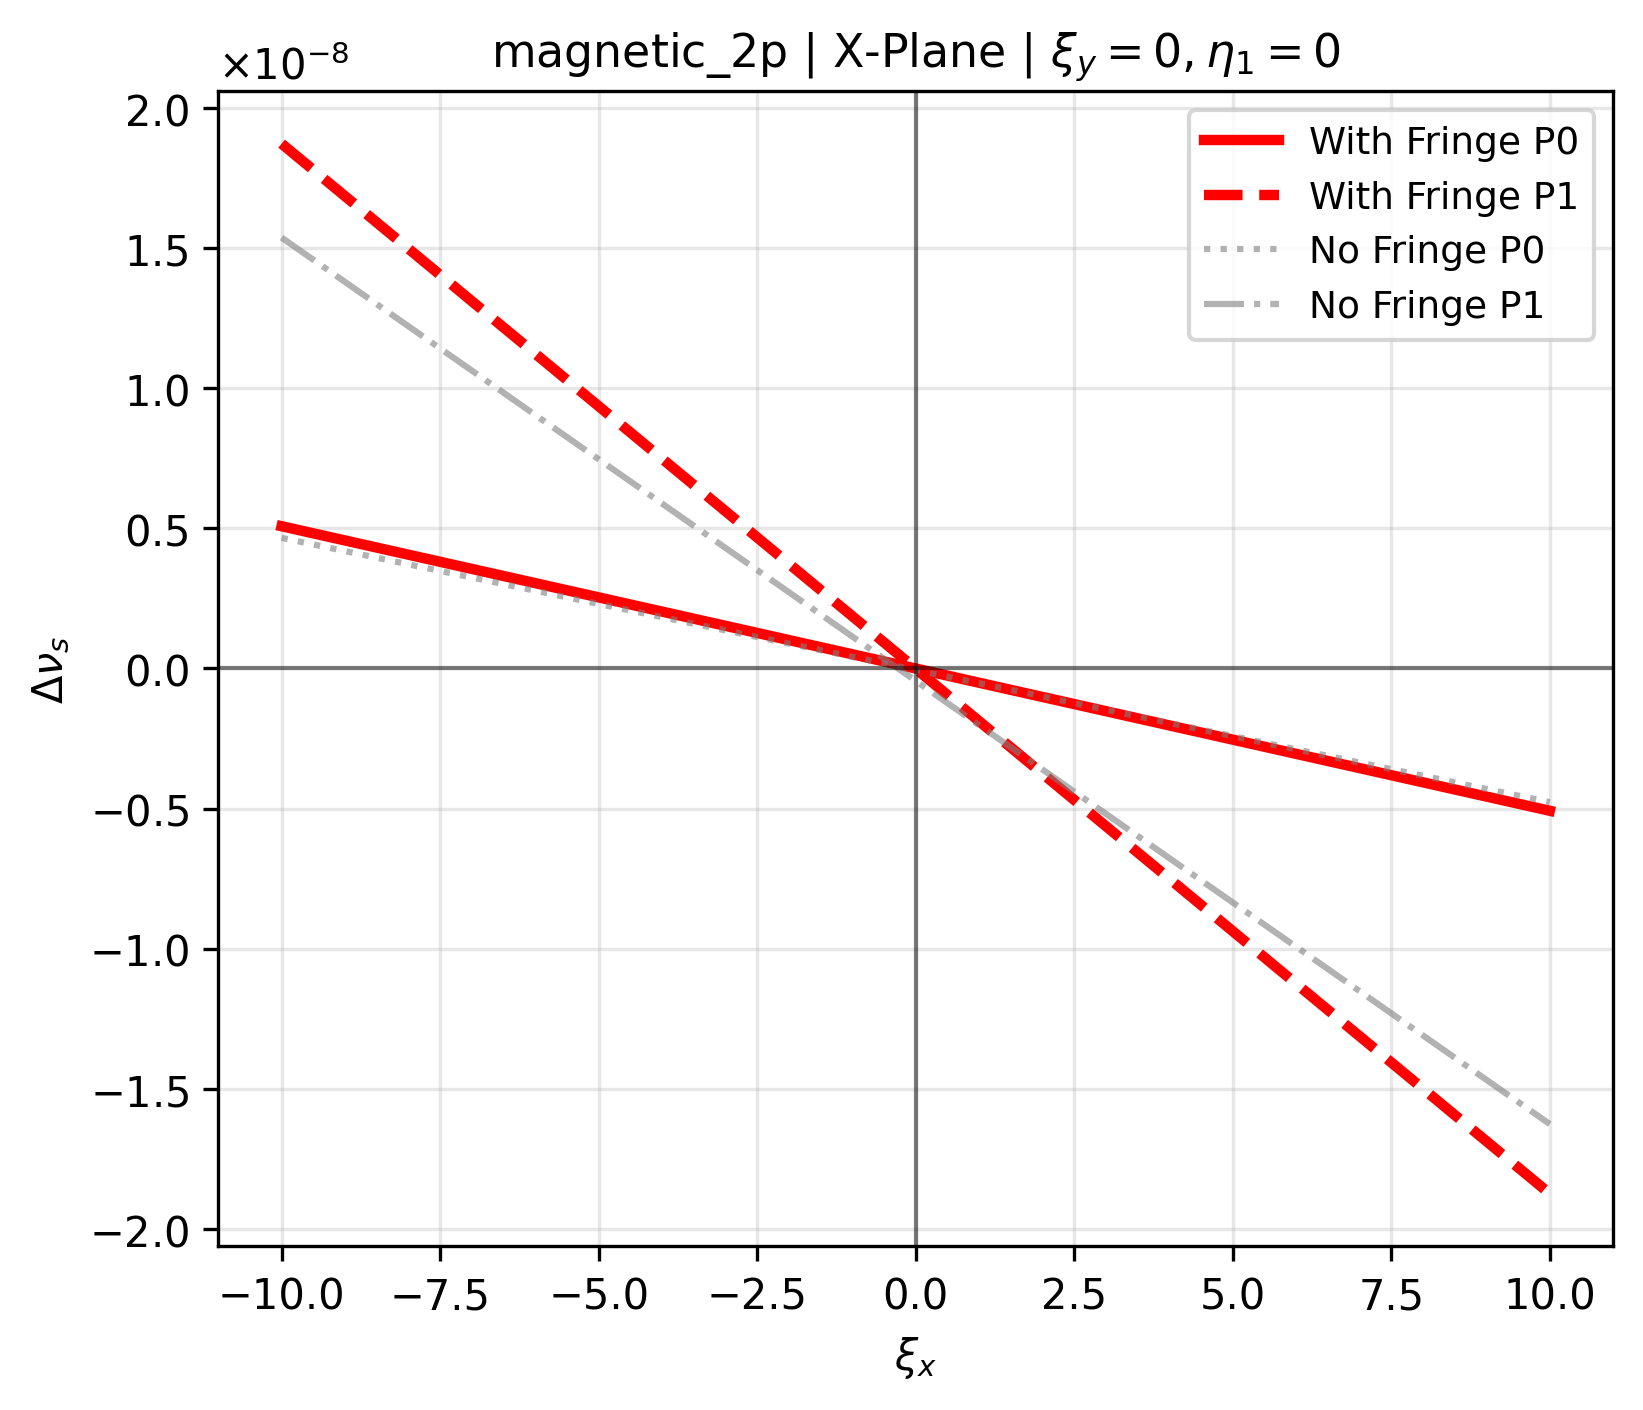
\includegraphics[width=0.95\hsize]{img/1483_f1}
	\caption{``magnetic\_2p'': \(\Delta\nu_s\) vs \(\xi_x\) at \(\xi_y=0,\,\eta_1=0\).}
	\label{fig:dual_x}
\end{figure}
\begin{figure}[!htb]
	\centering
	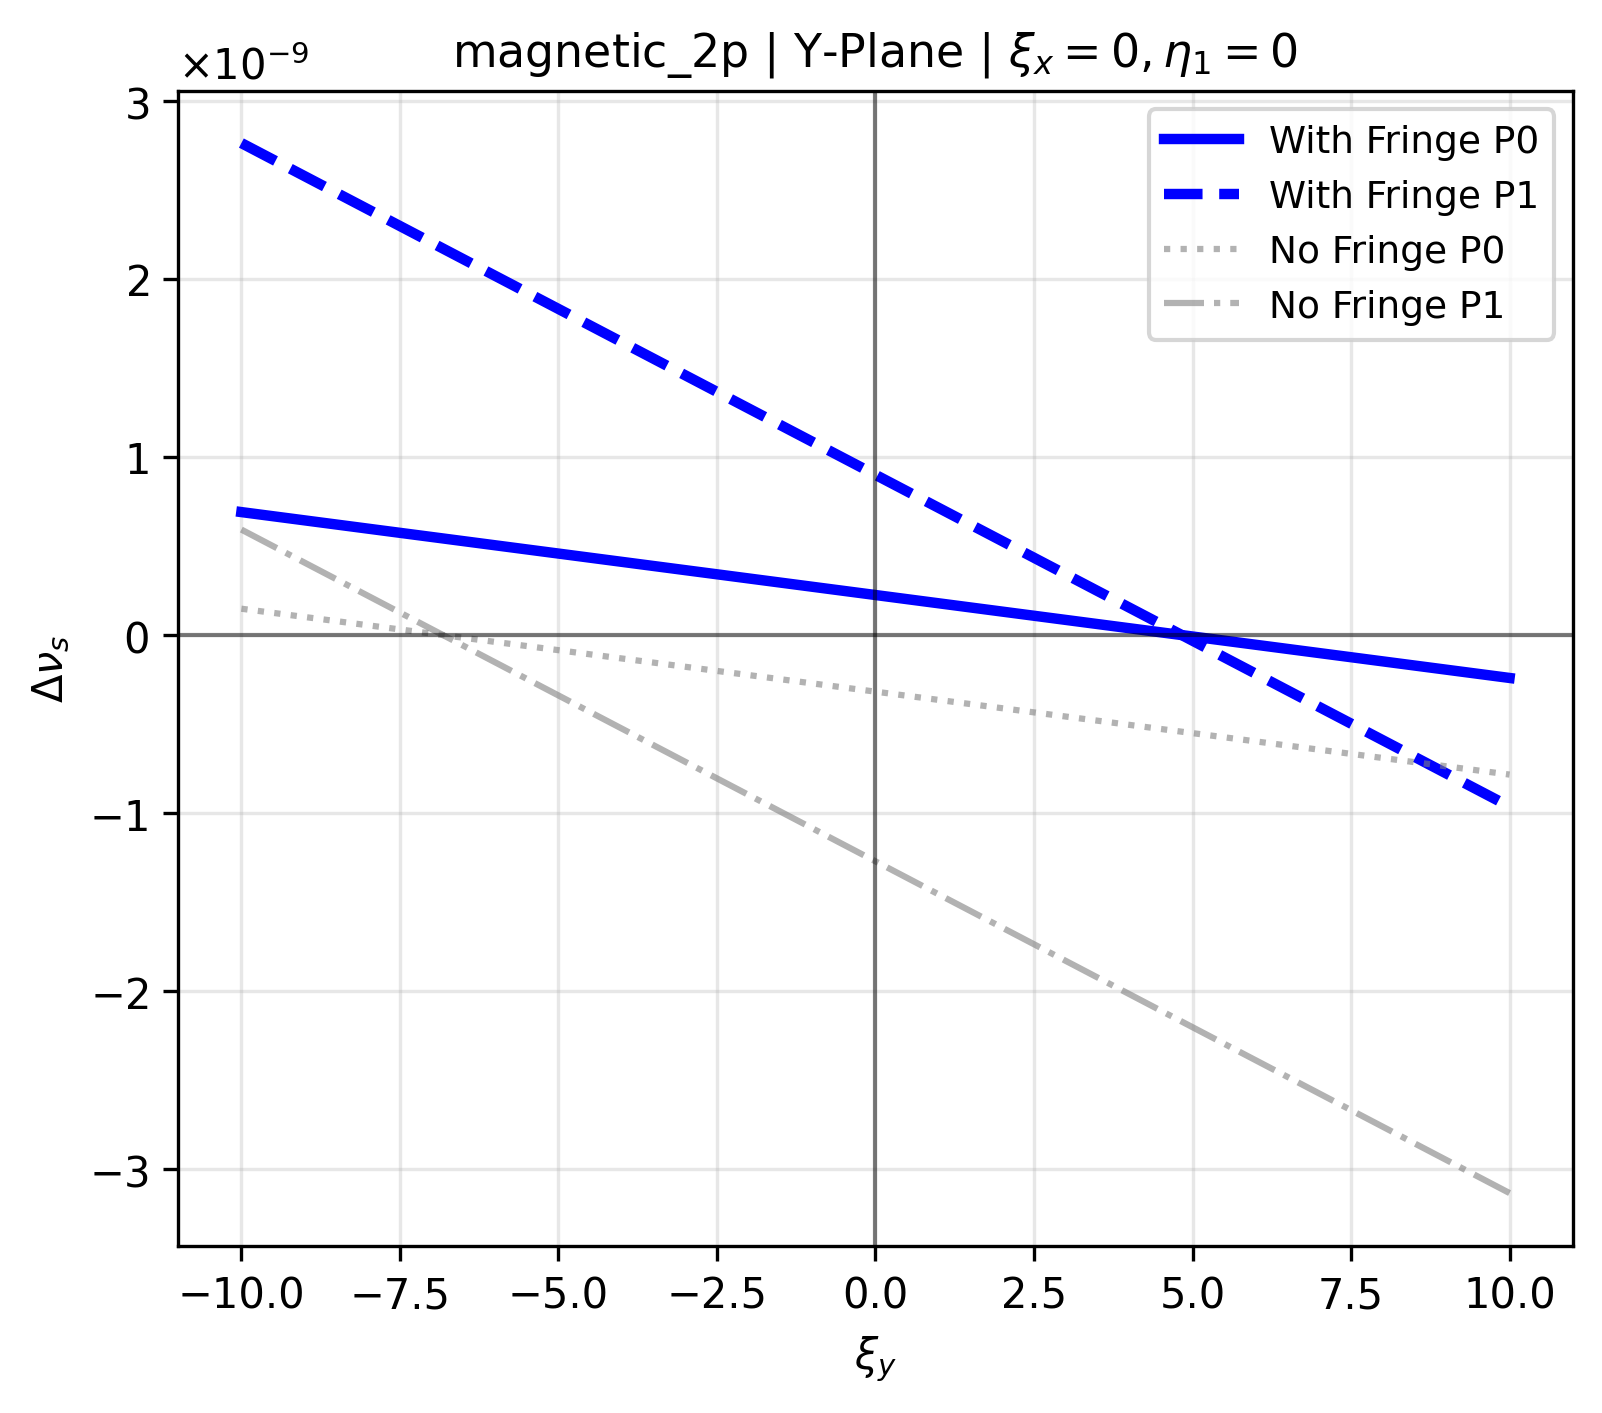
\includegraphics[width=0.95\hsize]{img/1483_f2}
	\caption{``magnetic\_2p'': \(\Delta\nu_s\) vs \(\xi_y\) at \(\xi_x=0,\,\eta_1=0\).}
	\label{fig:dual_y}
\end{figure}
\begin{figure}[!htb]
	\centering
	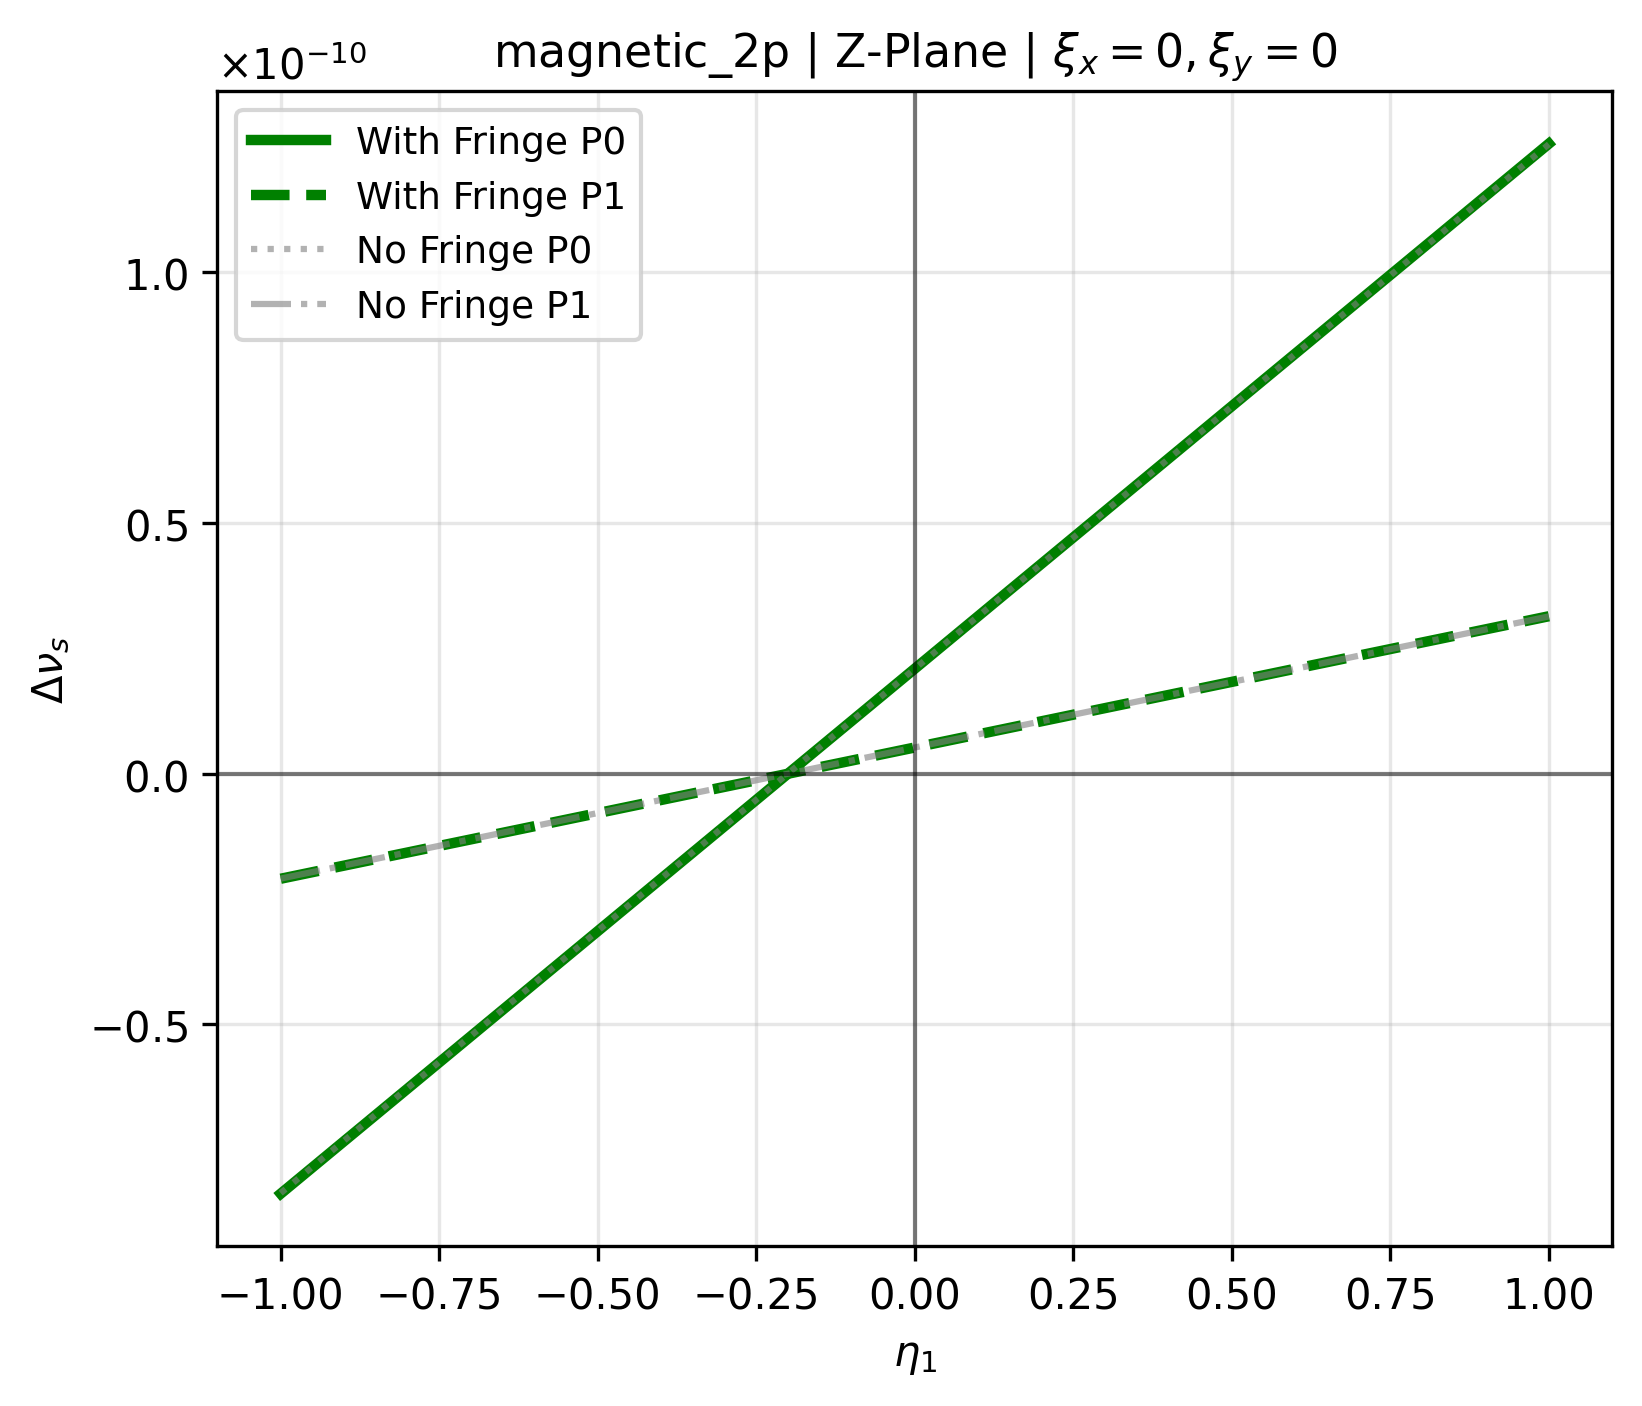
\includegraphics[width=0.95\hsize]{img/1483_f3}
	\caption{``magnetic\_2p'': \(\Delta\nu_s\) vs \(\eta_1\) at \(\xi_x=0,\,\xi_y=0\).}
	\label{fig:dual_z}
\end{figure}

\section{Results and discussion}
\par For each lattice, response matrices \(\mathbf{R}_{int}\) and \(\mathbf{R}_{spin}\) are built independently for two field representations (``No fringe'' and ``With fringe'') and for both probe amplitudes (P0 and P1). The comparison of resulting \(\mathbf{S}\) operators provides:
\begin{itemize}
	\item a quantitative measure of how realistic fringe fields distort the effective spin--chromaticity transfer;
	\item a non-linearity diagnostic through the difference between P0 and P1 responses;
	\item a practical tuning workflow, where sextupole settings are computed from Eq.~(\ref{eq:control_law}) while enforcing constraints in Eq.~(\ref{eq:constraints}).
\end{itemize}
\par A self-consistency check is performed by reconstructing sextupole settings from measured chromatic observables via Eq.~(\ref{eq:control_law}) and then predicting the spin response using Eq.~(\ref{eq:lin_model}), verifying that higher-order terms are small over the studied range.

\section{Conclusion}
\par A Jacobian-based mapping method for SCT-oriented sextupole tuning has been formulated and applied to a set of COSY-INFINITY lattice models. The approach provides an explicit spin--chromaticity transfer operator \(\mathbf{S}\) and supports constrained scans in \(\xi_x\), \(\xi_y\), and \(\eta_1\). The framework naturally incorporates comparisons between fringe/no-fringe field models and between nominal and large-amplitude probes, enabling a structured assessment of robustness and non-linear effects in SCT optimization.

\section{Acknowledgments}

\par A support of thus study by the Russian Science Foundation grant 25-72-30005 is acknowledged.

\ifboolexpr{bool{jacowbiblatex}}
	{\printbibliography}
	{
	\begin{thebibliography}{9}
	
	\bibitem{b1} A. D. Lehrach \emph{et al.}, ``Search for permanent electric dipole moments in storage rings,'' in {\it Proc. IPAC}, and references therein.
	\bibitem{b2} K. Makino and M. Berz, ``COSY INFINITY version 9,'' Nucl. Instrum. Methods Phys. Res. A {\bf 558} (2006) 346--350.
	\bibitem{b3} M. Berz, {\it Modern Map Methods in Particle Beam Physics}, Academic Press (1999).
	\bibitem{b4} S. Aksentyev \emph{et al.}, ``Spin coherence time studies with map-based techniques,'' internal report / work in progress.
	
	\end{thebibliography}
}

\end{document}